\section{Layout Recognition and OCR}
The first step in transforming the acquired book into a digital catalogue involved the identification and extraction of the article's structure and layout. This subsection outlines the process followed to achieve this goal.

\subsection{Structure Identification}
Initially, the book was obtained in a numeric scanned version, which presented the challenge of accurately identifying the structure and layout of the articles within its pages. Understanding the organization of the content was crucial for subsequent steps, such as extracting images, captions, and text blocks.

To tackle this task, an analysis of the book's structure and patterns was conducted. By visually examining the scanned pages, recurring patterns and common layouts were identified. These patterns included the arrangement of images, text blocks, headings, and other visual elements within the pages.

\subsection{Layout Model Training}
Various approaches were explored to automate the layout recognition process.
\subsubsection{Transkribus \parencite{transkribus}} 
Transkribus, a widely used tool for text recognition in historical documents, was initially considered for layout recognition.

Transkribus employs state-of-the-art machine learning techniques, such as convolutional neural networks (CNNs) and long short-term memory (LSTM) networks, to recognize and transcribe text from scanned documents.

In the case of the book's layout, Transkribus struggled to accurately identify and differentiate between images, captions, headings, and other visual components. The complexity and variation in layout structures posed a challenge to its inherent capabilities.

While Transkribus proved valuable for text recognition tasks, its limitations in layout recognition prompted the exploration of alternative methods.
By transitioning to a more tailored solution, the goal was to achieve accurate and comprehensive extraction of the book's layout elements, including both textual and non-textual components.

\subsubsection{Layout Parser}
To address the limitations encountered with Transkribus, the Layout Parser library was adopted as an alternative approach for layout recognition.

Layout Parser \parencite{shen2021layoutparser} is a Python library that provides a comprehensive set of tools and functionalities specifically designed for Deep Learning Based Document Image Analysis. It allows for the detection, extraction, and interpretation of various layout elements within scanned documents.

In the context of our book's layout recognition, the Layout Parser library offers a collection of pre-trained models on different datasets among which we chose PubLayNet. On top of being the largest dataset ever for document layout analysis, PubLayNet was the most adapted one to the book's structure. 
Among the models PubLayNet has been trained on, we chose Faster R-CNN: a deep convolutional network used for object detection.\\[0.3cm]


\begin{figure}[H]
    \centering
    \begin{minipage}[c]{.45\linewidth}
        \centering
        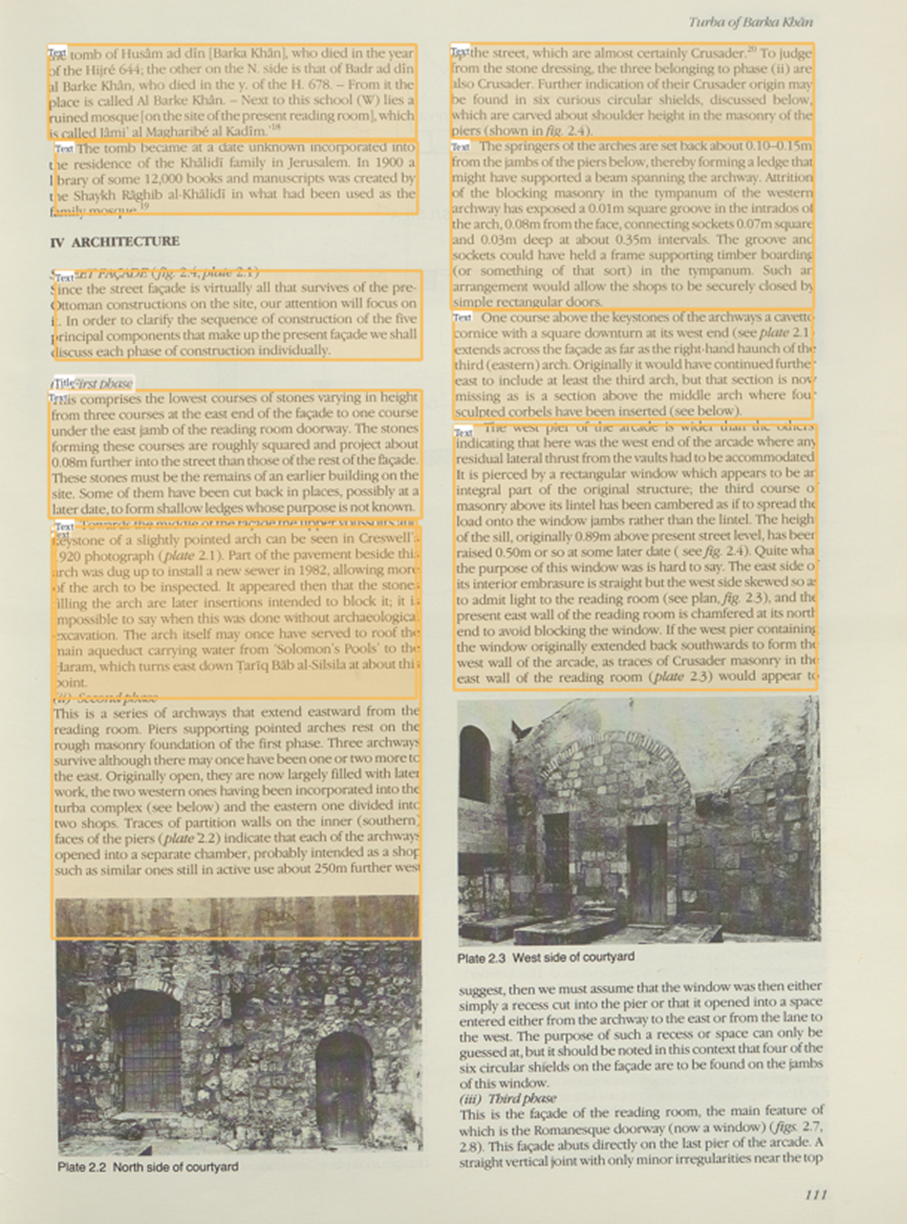
\includegraphics[width=0.9\textwidth]{Images/PLN4.png}
        \subcaption{Confidence: 0.8}
        \label{fig:Q40}
    \end{minipage}\hfill
    \begin{minipage}[c]{.45\linewidth}
        \centering
        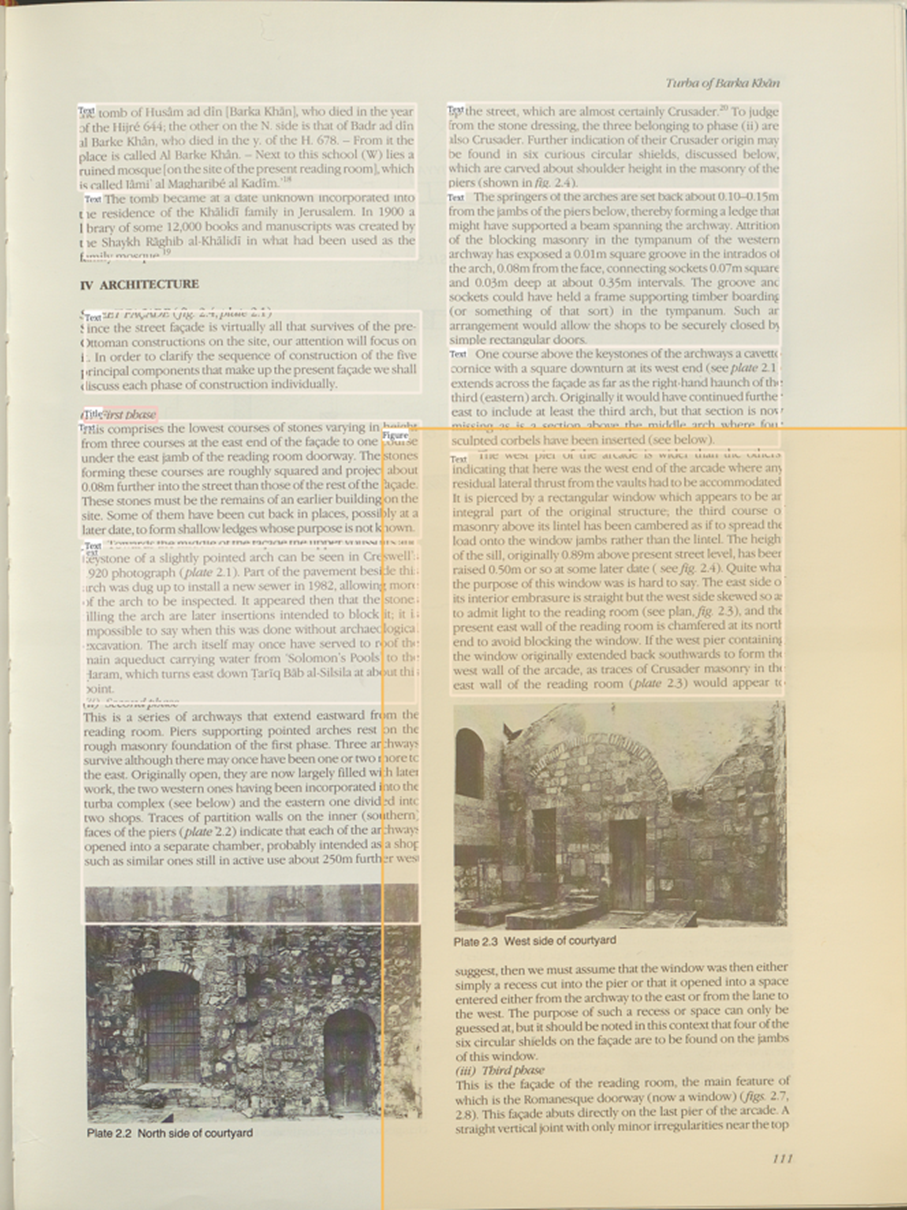
\includegraphics[width=0.9\textwidth]{Images/PLN8.png}
        \subcaption{Confidence: 0.4}
        \label{fig:Q41}
    \end{minipage}
    \caption{Layout Recognition with Faster R-CNN trained on PubLayNet}
    \label{fig:conf_comp}
\end{figure}

The \textbf{Figure \ref{fig:conf_comp}} shows that The results Layout Recognition with Faster R-CNN trained on PubLayNet. At a confidence threshold of 0.8, images were not even recognized, leading to incomplete or missing annotations. Similarly, at a confidence threshold of 0.4, the recognition of text and images was poor, resulting in inaccurate or imprecise bounding box placements. These limitations highlight the challenges faced in accurately identifying and extracting the layout using a pre-trained model.

As we will see later, training a layout model using additional annotated data was necessary for the model to learn the specific layout patterns and structures present in the book.

The goal was to accurately identify and extract different layout components, such as images, captions, headings, and text blocks, from the scanned book pages.

\subsubsection{Label Studio}
Label Studio \parencite{Label} is an open-source data annotation tool that provides a user-friendly interface allowing manual annotation of layout elements on images.
A total of 30 pages were selected, each page loaded individually into the annotation tool. \\[0.3cm]

\begin{figure}[H]
    \centering
    \scalebox{0.9} 
    {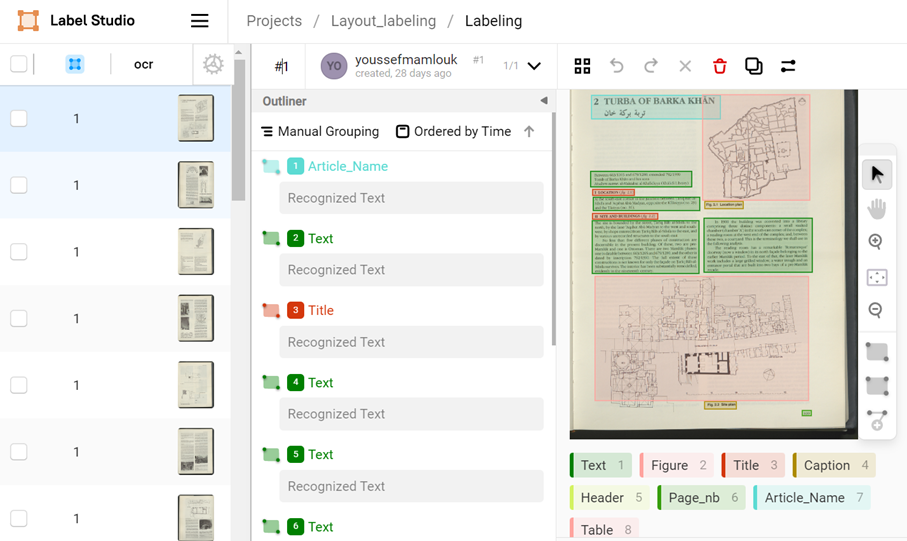
\includegraphics{Images/label_studio.png}}
    \caption{Manual annotation in Label Studio}
    \label{fig:label_studio}
\end{figure}

As we can see in the \textbf{Figure \ref{fig:label_studio}}, we were able to mark bounding boxes around various block components.
The chosen labels for annotation included:
\begin{itemize}
    \item "Article\_Name"
    \item "Text"
    \item "Title"
    \item "Caption"
    \item "Figure"
    \item "Header"
    \item "Page\_nb"
    \item "Table"
\end{itemize}

We wanted to be as precise as possible to facilitate data processing later.

The annotation process required careful attention to detail, consistency to ensure accurate labeling, and a good understanding of the book's structure and layout to minimize errors and inconsistencies in the annotations.

Label Studio allowed for more fine-grained control and customization of the layout recognition process, better suited to the book's specific layout complexities.
The annotated data was then exported in a COCO JSON \parencite{cocodataset}, a specific JSON structure (popular in Machine Learning) dictating how labels and metadata are saved for an image dataset, for further processing and training of the layout recognition model.

\subsubsection{Training}
The annotated data was split into two sets: a training set and a test set. The training set contained 85\% of the annotated pages, while the test set consisted of the rest used for evaluation.

The Layout Parser library, along with the annotated data, was used to train the layout recognition model. The model was trained using the already pre-trained weights of PubLayNet/Faster R-CNN. 

The training workflow consisted thus of fine-tuning the pre-trained model using the annotated data. \\[0.3cm]

\begin{figure}[H]
    \centering
    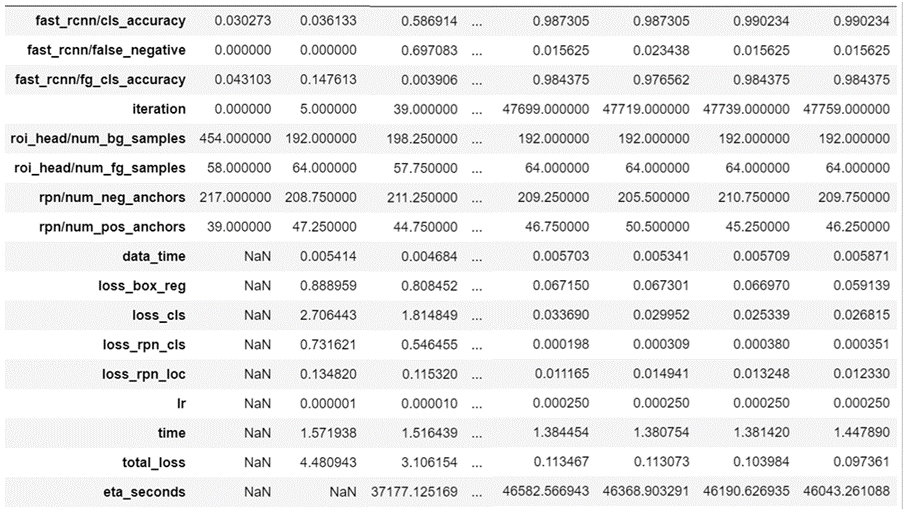
\includegraphics[width=0.9\textwidth]{Images/metrics.png}
    \caption{Training metrics over 47759 iterations}
    \label{fig:metrics}
\end{figure}

As we can see in the \textbf{Figure \ref{fig:metrics}}, this process was typically performed over multiple iterations for about 20 hours, where the model's parameters were updated based on the annotated data. Each epoch involved feeding the training data through the network, computing the loss, and updating the model's parameters to improve its performance.

\begin{figure}[H]
    \centering
    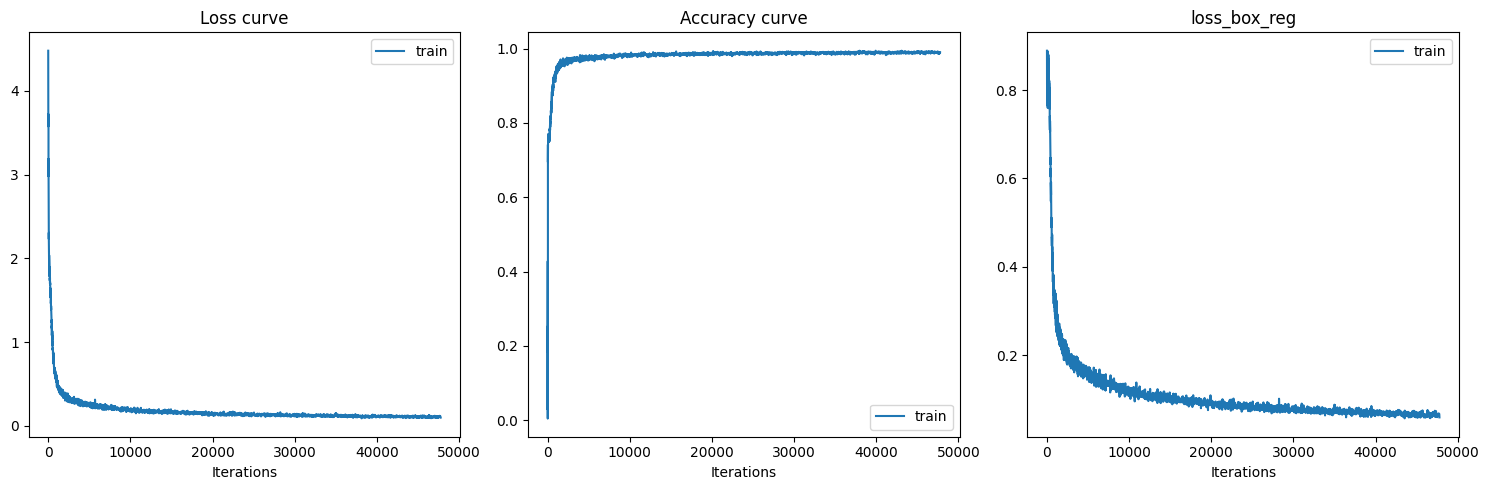
\includegraphics[width=0.99\textwidth]{Images/training_curves.png}
    \caption{Evolution of Total Loss, Accuracy and Bounding Box Loss through iterations}
    \label{fig:training}
\end{figure}

The training process was interrupted after 47,759 iterations as the loss and accuracy metrics reached a stable state, as evident from the plotted \textbf{Figures \ref{fig:training}}:
\begin{itemize}
    \item \textbf{Total Loss:} 0.097361
    \item \textbf{Accuracy:} 0.990234
    \item \textbf{Bounding Box Loss:} 0.059139
\end{itemize}

Continuing the training beyond this point would have provided minimal improvements to the model's performance. The observed stability in the loss curve and accuracy curve suggests that the model had already converged and further iterations would not yield significant enhancements. 

The goal of the training phase was to optimize the layout recognition model to accurately identify and extract layout components from the scanned book pages. The trained model would serve as a crucial component for subsequent steps in the transformation process, enabling the creation of a comprehensive digital catalogue.

\subsection{OCR}
After the layout recognition process, the next step was to initiate
the content extraction phase.
For this project, text extraction was the primary goal, as it provided the foundation for creating a comprehensive digital catalogue of the book's architectural content. The extracted text would be further processed, analyzed, and organized to enable efficient search, retrieval, and exploration of the architectural information.
However, during the extraction process, it was also possible to identify and extract images present in the scanned book pages. 
While these images contained valuable visual representations of the architectural elements, layout recognition did not perform as well as for textual content (see Layout Evaluation section).
They would have thus required additional post-training processing. Therefore, we decided to not use the extraction of images for the specific purpose of creating the digital catalogue. 

Instead, the emphasis was placed on extracting and processing the textual information using Optical Character Recognition (OCR) techniques. 
For this purpose, Tesseract, an open-source OCR engine, available within the Layout Parser library, was utilized.

Tesseract is a powerful OCR engine known for its accuracy and wide range of language support. It employs deep learning algorithms to recognize and extract text from images. The previously trained and fine-tuned layout recognition model, which accurately identified and localized text regions, played a crucial role in guiding the OCR process.

The OCR workflow involved the following steps:

\begin{itemize}
    \item \textbf{Preprocessing:} Before passing the extracted text regions to Tesseract for OCR, preprocessing techniques were applied to enhance the OCR accuracy. This mainly involved indexing text boxes in a properly sorted way so that they can be retrieved later in the correct order.
    \item \textbf{Text Region Extraction:} The layout recognition model, trained on the annotated data, provided precise bounding boxes around the text regions on the book pages. These bounding boxes were used to extract the text regions, ensuring that only the relevant text areas were processed.
    \item \textbf{OCR with Tesseract:} Text regions were then passed through Tesseract for OCR. Tesseract used deep learning models to analyze the images and convert them into machine-readable text. The recognized text was extracted along with its spatial coordinates to maintain its association with the layout structure.
    
\end{itemize}

The OCR process, combined with the layout recognition step, enabled the extraction of the textual content from the scanned book pages. The integration of Tesseract within the Layout Parser library facilitated a seamless and efficient workflow, allowing for accurate and reliable text extraction.

The extracted text data served as a crucial component for subsequent analysis, NLP (Natural Language Processing), and database management steps in the transformation process, enabling the creation of a comprehensive digital catalogue of the book's architectural content.


\section{Database Management}
The database management phase involved designing the database schema, cleaning the extracted text data, and inserting it into the database. 

\subsection{ER model}
The first step in designing the database was to create an Entity-Relationship (ER) model. The ER model served as a visual representation of the entities, attributes, and relationships within the data. 
It provided a high-level overview of the database structure, helping to identify the key entities and their associations.

During the ER modeling process (see \textbf{Figure \ref{fig:ER}}), the entities relevant to the architectural content and relationships between these were identified capturing the associations and dependencies among them.

We have chosen to structure articles into 6 entities:
\begin{itemize}
    \item \textbf{Building:} this is the main entity that has relations with every other one in the model. It represents each of the 64 Mamluk buildings and has an id as a primary key, a foreign key with every other entity (other than Inscription), a name, modern\_name and type attributes.
    \item \textbf{Location:} keeps track of the building's coordinates (longitude and latitude), the CRS (Coordinate Reference System), and id as a primary key and a description attribute that gives further textual details about the building's location.
    \item \textbf{Date:} that an id as a primary key, both hijri and gregorian dates as attributes, an explanation for the dates meaning (built, endowed,...) and 'others' attribute for further details about the date (taken from the history section).
    \item \textbf{History:} has id as primary key, identification, founder, endowments, and subsequent\_history information as attributes, a list of all subtitles of this section and others which loads the entire text of the History section in the article.
    \item \textbf{Architecture:} because of the complexity of this part's structure, we chose to simply store the entire text as well as the list of subtitles of the section in 'others' and 'subtitles' attributes respectively, and of course id as a primary key.
    \item \textbf{Inscription:} finally identifies all the inscriptions cited in the building's article. It has id as a primary key, the building reference stored in the foreign key 'building\_id', the inscription 'text', and a 'reference' for the section containing the inscription as attributes. \\[0.3cm]
\end{itemize}

\begin{figure}[H]
    \centering
    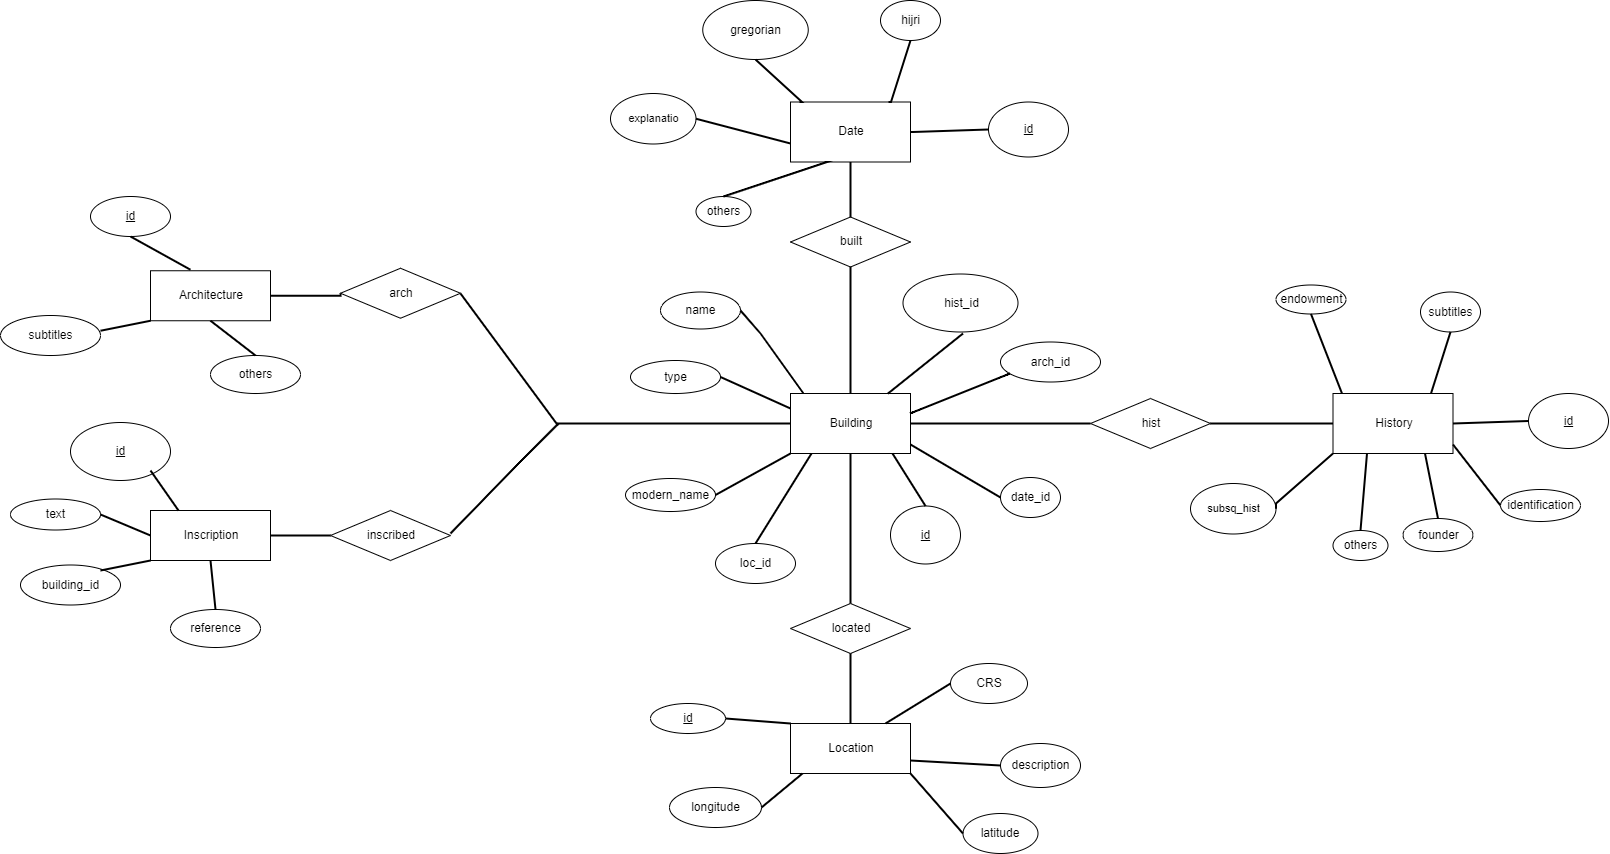
\includegraphics[width=0.9\textwidth]{Images/ER.png}
    \caption{ER Model of Mamluk buildings in Jerusalem}
    \label{fig:ER}
\end{figure}

The ER model acted as a blueprint for the subsequent creation of the relational model, which provided a more detailed representation of the database structure.

\subsection{Relational Model}
Based on the ER model, the next step was to convert it into a Relational Model. The Relational Model represented the database schema in the form of tables, with each table representing an entity and its corresponding attributes.

Using the identified entities and relationships from the ER model, tables were created in accordance with the principles of database normalization. The tables were designed to eliminate redundancy, ensure data integrity, and facilitate efficient data retrieval.

The attributes extracted from the OCR text were assigned to their respective tables and columns in the relational model we can observe in \textbf{Figure \ref{fig:rel_model}}.
The appropriate data types and constraints were defined to ensure the accuracy and consistency of the stored data. \\[0.3cm]

\begin{figure}[H]
    \centering
    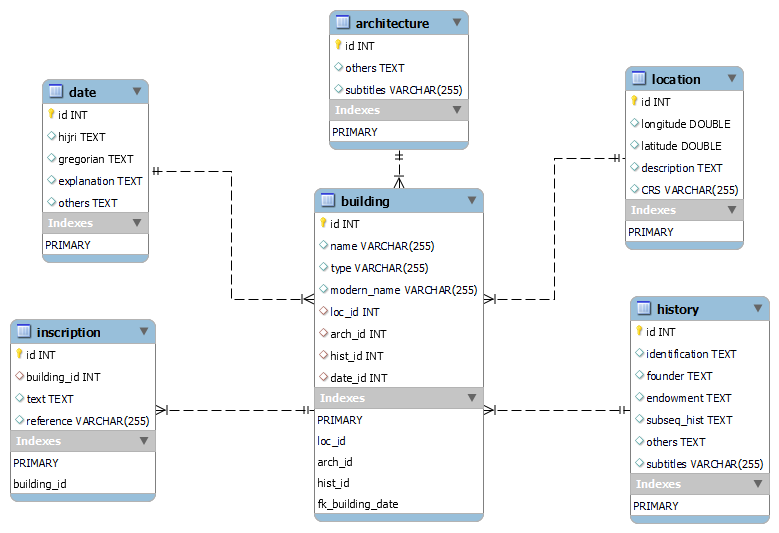
\includegraphics[width=0.8\textwidth]{Images/Rel_model.png}
    \caption{Relational Model}
    \label{fig:rel_model}
\end{figure}

\begin{figure}[H]
    \raisebox{-0.5\height}{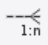
\includegraphics[width=0.05\textwidth]{Images/1_to_n.png}}
    \hspace{0.5em}  % Adjust the spacing as needed
    : representation of a 1 to n relation
    \label{fig:1_to_n}
\end{figure}



The Relational Model provided a structured and organized representation of the extracted text data, laying the foundation for the subsequent database insertion process.

\subsection{Database insertion}
\subsubsection{Data Cleaning}
Before inserting the extracted text data into the database, a data cleaning process was performed. This process aimed to preprocess and refine the raw text data to improve its quality and consistency.

Pandas, a powerful data manipulation library in Python, were used for data-cleaning tasks. The extracted text data was loaded into data frames, enabling efficient data transformation and manipulation.

NLP techniques from the NLTK (Natural Language Toolkit) library, were applied to perform tasks such as removing stopwords, punctuation, and special characters. Processes like stemming, using tools like the NLTK PortStemmer, were employed in some cases to reduce words to their root form, thereby reducing redundancy and improving data consistency.

The data cleaning process ensured that the text data was in a clean and standardized format, ready for insertion into the database.
\subsubsection{MySQL}
After data cleaning, the cleaned text data was inserted into a MySQL database. 
MySQL is an open-source relational database management system (RDBMS) widely used for storing, managing, and retrieving structured data. It has been chosen because it provides a reliable and efficient platform for data storage and offers robust features for data manipulation, querying, and indexing. 

The insertion process involved converting the data frames to CSV files, which served as an intermediate format for transferring the data to the database.

Using the csv python library, the data frames were converted to CSV files, ensuring that the data was structured in a tabular format suitable for insertion into the relational database. The CSV files were then used to generate SQL queries for database insertion.

The SQL queries were designed to create the necessary tables within the database schema and populate them with the cleaned text data. The INSERT statements were executed to insert the data into the appropriate tables and columns.

By leveraging the capabilities of Pandas, Python, and MySQL, the text data was effectively transformed and loaded into the database. This allowed for efficient storage, management, and retrieval of the architectural content within the digital catalogue.

The successful completion of the database insertion process established a solid foundation for further data management and facilitated the seamless integration of the extracted text data into the digital catalogue system.

\section{Data visualization}
The data visualization phase aimed to present the extracted architectural data in an interactive and visually appealing manner. The chosen approach involved creating an interactive leaflet map that displayed Mamluk buildings and provided various ways to interact with each building. The section below provides further details on the data visualization process.

The initial approach to implementing the interactive map was to utilize the Folium Python library \parencite{folium}. Folium offers map visualization capabilities, allowing for the integration of geographical data with interactive elements. However, during the implementation phase, limitations in interactivity were encountered, prompting a switch to the ipyleaflet library.

The ipyleaflet library \parencite{ipyleaflet}, a Jupyter-friendly Python library based on the Leaflet JavaScript library, was chosen as an alternative due to its enhanced interactivity features and compatibility with Jupyter notebooks. ipyleaflet provided a powerful framework for creating interactive maps with customizable markers and interactive controls.

By leveraging the ipyleaflet library, the focus was on developing an interactive leaflet map that showcased the Mamluk buildings. Each building would be represented as a marker on the map, visually indicating its location. Additionally, various interactive elements were incorporated to enhance the user experience and provide additional information about each building.

The map's interactivity allowed users to interact with the markers and access detailed information about specific buildings. For example, clicking on a marker could trigger a pop-up window displaying information such as the building's name, historical significance, architectural features, and related inscriptions. Zooming and panning functionality enabled users to explore the map at different scales and navigate through different regions of interest.

The results section will provide a comprehensive demonstration and analysis of the interactive features and functionalities of the leaflet map. It will showcase how map visualization and interactivity contribute to a better understanding and exploration of the Mamluk buildings in Jerusalem, enriching the overall digital catalogue experience.

